% lecture09.tex — Manifolds with Boundary

\section{Manifolds with Boundary}

Consider the closed \emph{half-space}
\[
    H^m := \{(x_1, \ldots, x_m) \in \R^m \mid x_m \geq 0\}.
\]
The boundary $\partial H^m$ is defined to be the hyperplane $\R^{m-1} \times 0 \subset \R^m$.

\begin{definition}{Manifold with Boundary}{manifold-boundary}
    A subset $M \subset \R^k$ is called a \emph{smooth $m$-manifold with boundary} if it is locally diffeomorphic to $H^m$.
\end{definition}

The \emph{boundary} $\partial M$ is the set of all points of $M$ which correspond to points of $\partial H^m$ under such a local parametrization. Its complement is called the \emph{interior} $\operatorname{Int}(M) = M - \partial M$.

\begin{center}
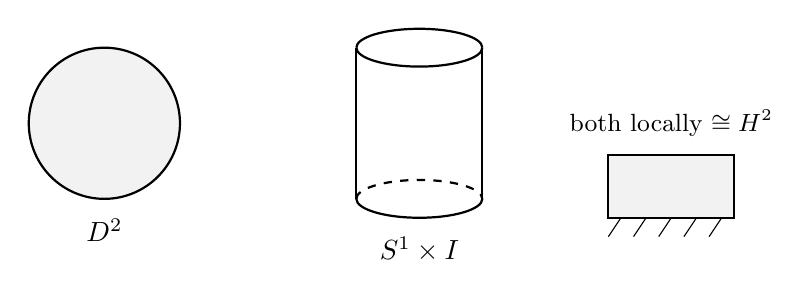
\begin{tikzpicture}[scale=0.8]
    % Disk D^2
    \draw[thick,fill=gray!10] (0,0) circle (1.2);
    \node at (0,-1.7) {$D^2$};
    % Cylinder S^1 x I
    \begin{scope}[xshift=5cm]
        \draw[thick] (-1,1.2) -- (-1,-1.2);
        \draw[thick] (1,1.2) -- (1,-1.2);
        \draw[thick] (-1,1.2) arc(180:360:1 and 0.3);
        \draw[thick] (-1,1.2) arc(180:0:1 and 0.3);
        \draw[thick] (-1,-1.2) arc(180:360:1 and 0.3);
        \draw[thick,dashed] (-1,-1.2) arc(180:0:1 and 0.3);
        \node at (0,-2) {$S^1 \times I$};
    \end{scope}
    % Label
    \node at (9,0) {\small both locally $\cong H^2$};
    % H^2
    \begin{scope}[xshift=9cm,yshift=-1.5cm]
        \draw[thick,fill=gray!10] (-1,0) rectangle (1,1);
        \draw[thick] (-1,0) -- (1,0);
        \foreach \x in {-0.8,-0.4,0,0.4,0.8} {
            \draw (\x,0) -- (\x-0.2,-0.3);
        }
    \end{scope}
\end{tikzpicture}
\end{center}

\begin{proposition}{Boundary is a Manifold}{boundary-manifold}
    If $M$ is a smooth $m$-manifold with boundary, $\partial M$ is a well-defined smooth $(m-1)$-manifold (without boundary).
\end{proposition}

\begin{proof}
    For any open neighborhood $U$ of $x \in \partial H^m$ in $H^m$, $U \cap \partial H^m$ is an open subset of $\partial H^m \cong \R^{m-1}$, so it suffices to show that any diffeomorphism between open subsets of $H^m$ sends boundary points to boundary points.

    Suppose $f \colon U \to V$ is such a diffeomorphism, and that it maps some $x \in \partial U$ to an interior point $y = f(x)$ of $V$. But then $f^{-1}$ must map an open neighborhood of $y$ in $\R^m$ (contained in $V$) onto an open neighborhood of $x$ in $\R^m$, which contradicts $x \in \partial U$.

    Therefore, $\partial M$ is a well-defined smooth $(m-1)$-manifold.
\end{proof}

The \emph{tangent space} $T_p M$ is defined just as before, so that it is a full $m$-dimensional vector space, even if $p \in \partial M$. In case $p \in \partial M$, there is a natural inclusion $T_p(\partial M) \hookrightarrow T_p M$ ($(m-1)$-dimensional into $m$-dimensional).

\begin{center}
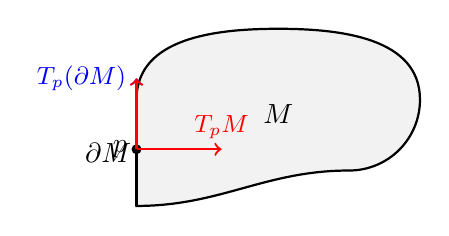
\begin{tikzpicture}[scale=0.9]
    % Manifold M with boundary
    \draw[thick,fill=gray!10] (0,0) to[out=0,in=180] (3,0.5) to[out=0,in=270] (4,1.5) to[out=90,in=0] (2,2.5) to[out=180,in=90] (0,1.5) -- cycle;
    \draw[very thick] (0,0) -- (0,1.5);
    \node at (2,1.3) {$M$};
    \node at (-0.4,0.75) {$\partial M$};
    % Point on boundary
    \fill (0,0.8) circle (2pt) node[left] {$p$};
    % T_p(∂M) — vertical
    \draw[->,thick,blue] (0,0.8) -- (0,1.8) node[left] {\small $T_p(\partial M)$};
    % T_pM — extends into M
    \draw[->,thick,red] (0,0.8) -- (1.2,0.8) node[above] {\small $T_p M$};
    \draw[->,thick,red] (0,0.8) -- (0,1.8);
\end{tikzpicture}
\end{center}

\subsection{Generating Examples}

Here's one method for generating examples:

\begin{lemma}{Preimage of a Regular Value}{preimage-boundary}
    Let $M$ be a manifold (without boundary) and let $g \colon M \to \R$ have $0$ as a regular value. Then $\{x \in M \mid g(x) \geq 0\}$ is a smooth manifold with boundary $g^{-1}(0)$.
\end{lemma}

\begin{proof}
    The set where $g > 0$ is open in $M$ and hence a submanifold of the same dimension. At points of $g^{-1}(0)$, $g$ is locally equivalent to the canonical submersion, and the lemma is obvious.
\end{proof}

\begin{example}{Unit Disk}{unit-disk}
    The unit disk $D^m = \{x \in \R^m \mid 1 - \sum_{i=1}^m x_i^2 \geq 0\}$ is a smooth manifold with boundary $\partial D^m = S^{m-1}$.
\end{example}

\subsection{Preimage Theorem with Boundary}

We also have a version of the preimage theorem:

\begin{theorem}{Preimage Theorem for Manifolds with Boundary}{preimage-boundary-thm}
    Let $f \colon M \to N$ be a smooth map from a manifold $M$ with boundary to a manifold $N$ (without boundary), and suppose that both $f \colon M \to N$ and $\partial f := f|_{\partial M} \colon \partial M \to N$ are transversal with respect to a submanifold $P \subset N$.

    Then, $f^{-1}(P) \subset M$ is a manifold with boundary $\partial f^{-1}(P) = f^{-1}(P) \cap \partial M$, and $\codim(f^{-1}(P) \subset M) = \codim(P \subset N)$.
\end{theorem}

\begin{proof}
    We only need to examine $f^{-1}(P)$ in a neighborhood of a point $x \in f^{-1}(P) \cap \partial M$, thanks to the earlier preimage theorem.

    As usual, in some neighborhood of $y = f(x) \in P$, there's a submersion $g$ to $\R^\ell$, $\ell = \codim(P \subset N)$, such that $P = g^{-1}(0)$ in this neighborhood.

    \begin{center}
    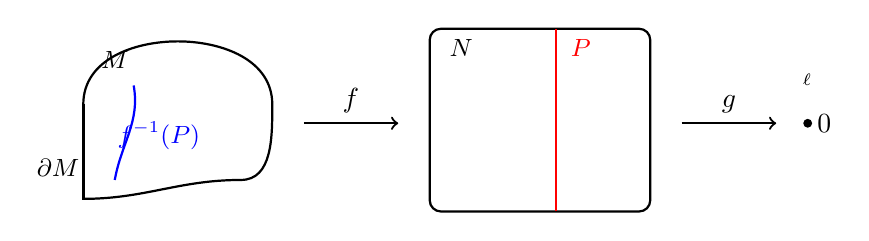
\begin{tikzpicture}[scale=0.8]
        % M with boundary, f^{-1}(P)
        \draw[thick] (0,0) to[out=0,in=180] (2.5,0.3) to[out=0,in=270] (3,1.5) to[out=90,in=0] (1.5,2.5) to[out=180,in=90] (0,1.5) -- cycle;
        \draw[very thick] (0,0) -- (0,1.5);
        \node at (0.5,2.2) {\small $M$};
        \node at (-0.4,0.5) {\small $\partial M$};
        \draw[thick,blue] (0.5,0.3) to[out=80,in=280] (0.8,1.8);
        \node[blue] at (1.2,1) {\small $f^{-1}(P)$};
        % Arrow
        \draw[->,thick] (3.5,1.2) -- (5,1.2) node[midway,above] {$f$};
        % N with P
        \draw[thick,rounded corners] (5.5,-0.2) rectangle (9,2.7);
        \node at (6,2.4) {\small $N$};
        \draw[thick,red] (7.5,-0.2) -- (7.5,2.7);
        \node[red] at (7.9,2.4) {\small $P$};
        % Arrow g
        \draw[->,thick] (9.5,1.2) -- (11,1.2) node[midway,above] {$g$};
        \fill (11.5,1.2) circle (2pt) node[right] {$0$};
        \node at (11.5,1.8) {\small $\R^\ell$};
    \end{tikzpicture}
    \end{center}

    Pre-composing with a local parametrization $\phi \colon U \subset H^m \to M$ around $x$, we obtain a map $h = g \circ f \circ \phi \colon U \subset H^m \to \R^\ell$ which is a submersion. By definition of smoothness, $h$ extends to a smooth map $\tilde{h}$ defined on a neighborhood $\tilde{U}$ of $u$ in $\R^m$, and the preimage $\tilde{h}^{-1}(0) \subset \tilde{U}$ is a manifold.

    Now, the transversality assumption on $\partial f$ implies that the last coordinate $x_m$ is regular on $\tilde{h}^{-1}(0)$ at $u$. Therefore, by the previous lemma, $\tilde{h}^{-1}(0) \cap \{x_m \geq 0\}$ is a manifold with boundary $\tilde{h}^{-1}(0) \cap \{x_m = 0\}$.
\end{proof}
